\chapter{Results}
\label{chap:results}
\section{Eye-traker Data}
The study developed in python has proven interesting results regarding the 
metrics mentioned in chapter \ref{chap:data_analysis}. The results will show the results of the statistics along with
the basic statistical values such as mean and standard deviation.
\subsection{Total Duration of Whole Fixations}
Table \ref{tab:tdwf_basic_stats} shows that the mean was higher in length for positive polarity in all TOIs,
having the biggest difference in the Wiki-Based Scene.
\begin{table}[H]
    \centering
    \small
    \setlength{\tabcolsep}{4pt}
    \renewcommand{\arraystretch}{1.3}
    \caption{Results of Total Duration of Whole Fixations}
    \label{tab:tdwf_basic_stats}

    \resizebox{0.98\linewidth}{!}{
    \begin{tabular}{|c|c|c|c|c|c|}
        \hline
        \textbf{Display Polarity} & \textbf{TOI} & \shortstack{\textbf{Min.} \\ \textbf{(ms)}} & \shortstack{\textbf{Mean} \\ \textbf{(ms)}} & \shortstack{\textbf{Std.} \\ \textbf{Deviation} \\ \textbf{(ms)}} & \shortstack{\textbf{Max.} \\ \textbf{(ms)}} \\ \hline
        

        \multirow{3}{*}{Positive Polarity} & \textbf{Wiki-based} & 18570 & 52902.88 & 24410.26 & 125026 \\ \cline{2-6}
         & \textbf{E-Commerce} & 9443 & 64217.12 & 34024.20 & 125642 \\ \cline{2-6}
         & \textbf{Entire Exp.} & 215011 & 347509 & 81449.08 & 504168 \\ \hline
        

        \multirow{3}{*}{Negative Polarity} & \textbf{Wiki-based} & 2631 & 41879.59 & 17204.72 & 72631 \\ \cline{2-6}
         & \textbf{E-Commerce} & 8977 & 53989.41 & 22480.35 & 94915 \\ \cline{2-6}
         & \textbf{Entire Exp.} & 154088 & 282626.65 & 63197.95 & 391933 \\ \hline
    \end{tabular}
    }
\end{table}
Figure \ref{fig:tdwf_boxplot} shows how only the entire experiment has significant results within this variable. 
Further statistics can be seen in table \ref{tab:tdwf_stats} where p-values under $\alpha=0.05$ are highlighted in 
red and p-values under $\alpha=0.1$ are highlighted in orange. 
\begin{figure}[H]
    \centering
    \includegraphics[width=0.8\textwidth]{figures/Total_Duration_of_Whole_Fixations.png}
    \caption{Total Duration of Fixations for each Display Polarity and TOI.}
    \label{fig:tdwf_boxplot}
\end{figure}

\begin{table}[H]
    \centering
    \small
    \setlength{\tabcolsep}{4pt}
    \caption{Statistics of Total Duration of Whole Fixations}
    \label{tab:tdwf_stats}
    \resizebox{0.98\linewidth}{!}{
    \begin{tabular}{|c|c|c|c|c|}
        \hline
        \textbf{TOI} & \textbf{W\textsubscript{PP}} & \textbf{W\textsubscript{NP}} & \textbf{T-Student} & \textbf{Mann-Whitney} \\ \hline
        Wiki-Based & \textbf{\color{red}0.0091} & 0.7774 & - & 0.2557 \\ \hline
        E-Commerce & 0.7094 & 0.9138 & 0.3244 & - \\ \hline
        Entire Exp. & 0.8348 & 0.9790 & \textbf{\color{red}0.0174} & - \\ \hline
    \end{tabular}
    }
\end{table}

\subsection{Total Number of Fixations}
Regarding the total number of fixations, table \ref{tab:tnf_basic_stats} proves that the mean number of fixations 
is higher in positive polarity in every single TOI.
\begin{table}[H]
    \centering
    \small
    \setlength{\tabcolsep}{4pt}
    \renewcommand{\arraystretch}{1.3}
    \caption{Results of Total Number of Fixations}
    \label{tab:tnf_basic_stats}

    \resizebox{0.98\linewidth}{!}{
    \begin{tabular}{|c|c|c|c|c|c|}
        \hline
        \textbf{Display Polarity} & \textbf{TOI} & \shortstack{\textbf{Min.}} & \shortstack{\textbf{Mean}} & \shortstack{\textbf{Std.} \\ \textbf{Deviation}} & \shortstack{\textbf{Max.}} \\ \hline
        

        \multirow{3}{*}{Positive Polarity} & \textbf{Wiki-based} & 62 & 158.94 & 52.41 & 301 \\ \cline{2-6}
         & \textbf{E-Commerce} & 35 & 199.06 & 92.76 & 320 \\ \cline{2-6}
         & \textbf{Entire Exp.} & 545 & 979.59 & 240.28 & 1510 \\ \hline
        

        \multirow{3}{*}{Negative Polarity} & \textbf{Wiki-based} & 13 & 142.65 & 50.59 & 208 \\ \cline{2-6}
         & \textbf{E-Commerce} & 45 & 194.06 & 64.46 & 280 \\ \cline{2-6}
         & \textbf{Entire Exp.} & 405 & 844.82 & 162.51 & 1159\\ \hline
    \end{tabular}
    }
\end{table}
The statistical analysis, as seen in figure \ref{fig:tnf_boxplot} and table \ref{tab:tnf_stats}. There is no
significant difference between both groups but the entire experiment is close to be significant with a p-value of 0.0736 in the T-Student test.
\begin{figure}[H]
    \centering
    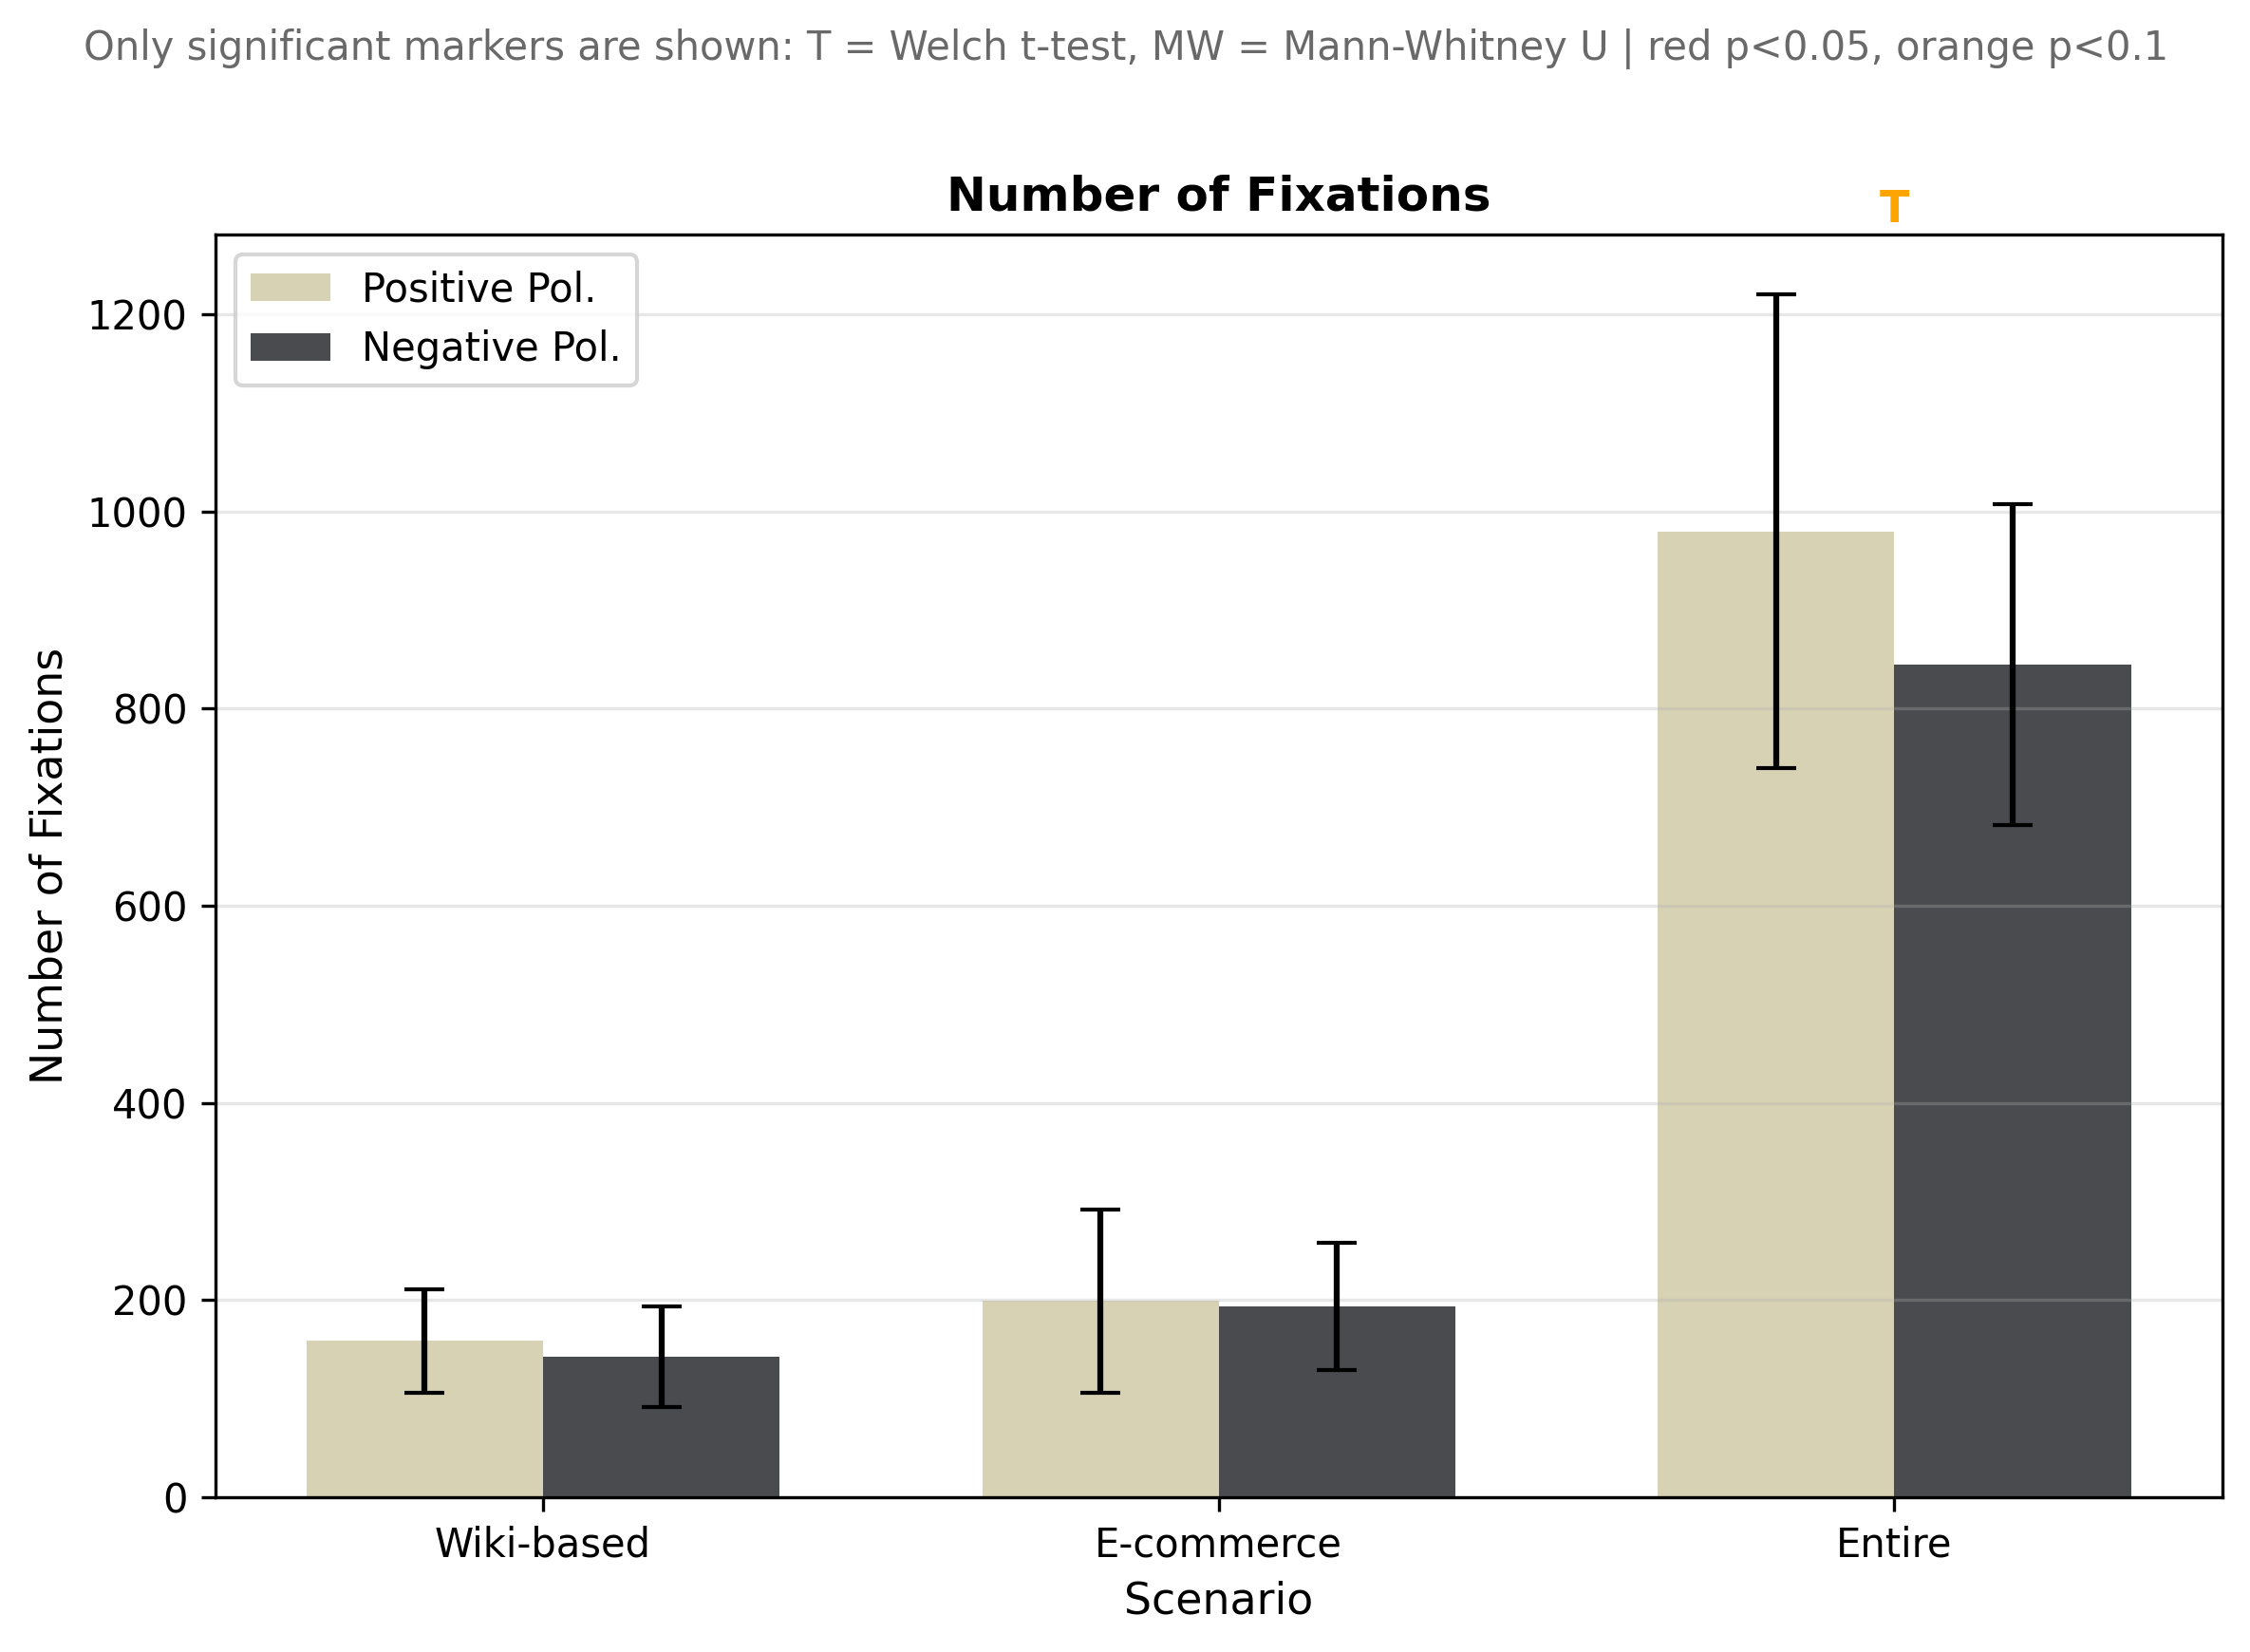
\includegraphics[width=0.8\textwidth]{figures/Number_of_whole_fixations.png}
    \caption{Total Number of Fixations for each Display Polarity and TOI.}
    \label{fig:tnf_boxplot}
\end{figure}

\begin{table}[H]
    \centering
    \small
    \setlength{\tabcolsep}{4pt}
    \caption{Statistics of Total Number of Fixations}
    \label{tab:tnf_stats}
    \resizebox{0.98\linewidth}{!}{
    \begin{tabular}{|c|c|c|c|c|}
        \hline
        \textbf{TOI} & \textbf{W\textsubscript{PP}} & \textbf{W\textsubscript{NP}} & \textbf{T-Student} & \textbf{Mann-Whitney} \\ \hline
        Wiki-Based & 0.5150 & 0.2003 & 0.3776 & - \\ \hline
        E-Commerce & 0.1019 & 0.1089 & 0.8591 & - \\ \hline
        Entire Exp. & 0.5321 & 0.3570 & \textbf{\color{orange}0.0736} & - \\ \hline
    \end{tabular}
    }
\end{table}

\subsection{Duration of First Fixation}
The first duration of fixation is lower in positive polarity in both TOIS but differs in the whole recording,
as shown in table \ref{tab:dfff_basic_stats}. 
\begin{table}[H]
    \centering
    \small
    \setlength{\tabcolsep}{4pt}
    \renewcommand{\arraystretch}{1.3}
    \caption{Results of Duration of First Fixation}
    \label{tab:dfff_basic_stats}

    \resizebox{0.98\linewidth}{!}{
    \begin{tabular}{|c|c|c|c|c|c|}
        \hline
        \textbf{Display Polarity} & \textbf{TOI} & \shortstack{\textbf{Min.} \\ \textbf{(ms)}} & \shortstack{\textbf{Mean} \\ \textbf{(ms)}} & \shortstack{\textbf{Std.} \\ \textbf{Deviation} \\ \textbf{(ms)}} & \shortstack{\textbf{Max.} \\ \textbf{(ms)}} \\ \hline
        

        \multirow{3}{*}{Positive Polarity} & \textbf{Wiki-based} & 83 & 181.21 & 111.99 & 583 \\ \cline{2-6}
         & \textbf{E-Commerce} & 133 & 193 & 54.03 & 316 \\ \cline{2-6}
         & \textbf{Entire Exp.} & 67 & 315.47 & 268.45 & 1016 \\ \hline
        

        \multirow{3}{*}{Negative Polarity} & \textbf{Wiki-based} & 100 & 205.82 & 100.07 & 533 \\ \cline{2-6}
         & \textbf{E-Commerce} & 83 & 200 & 123.55 & 650 \\ \cline{2-6}
         & \textbf{Entire Exp.} & 67 & 203.88 & 163.85 & 766 \\ \hline
    \end{tabular}
    }
\end{table}
\begin{figure}[H]
    \centering
    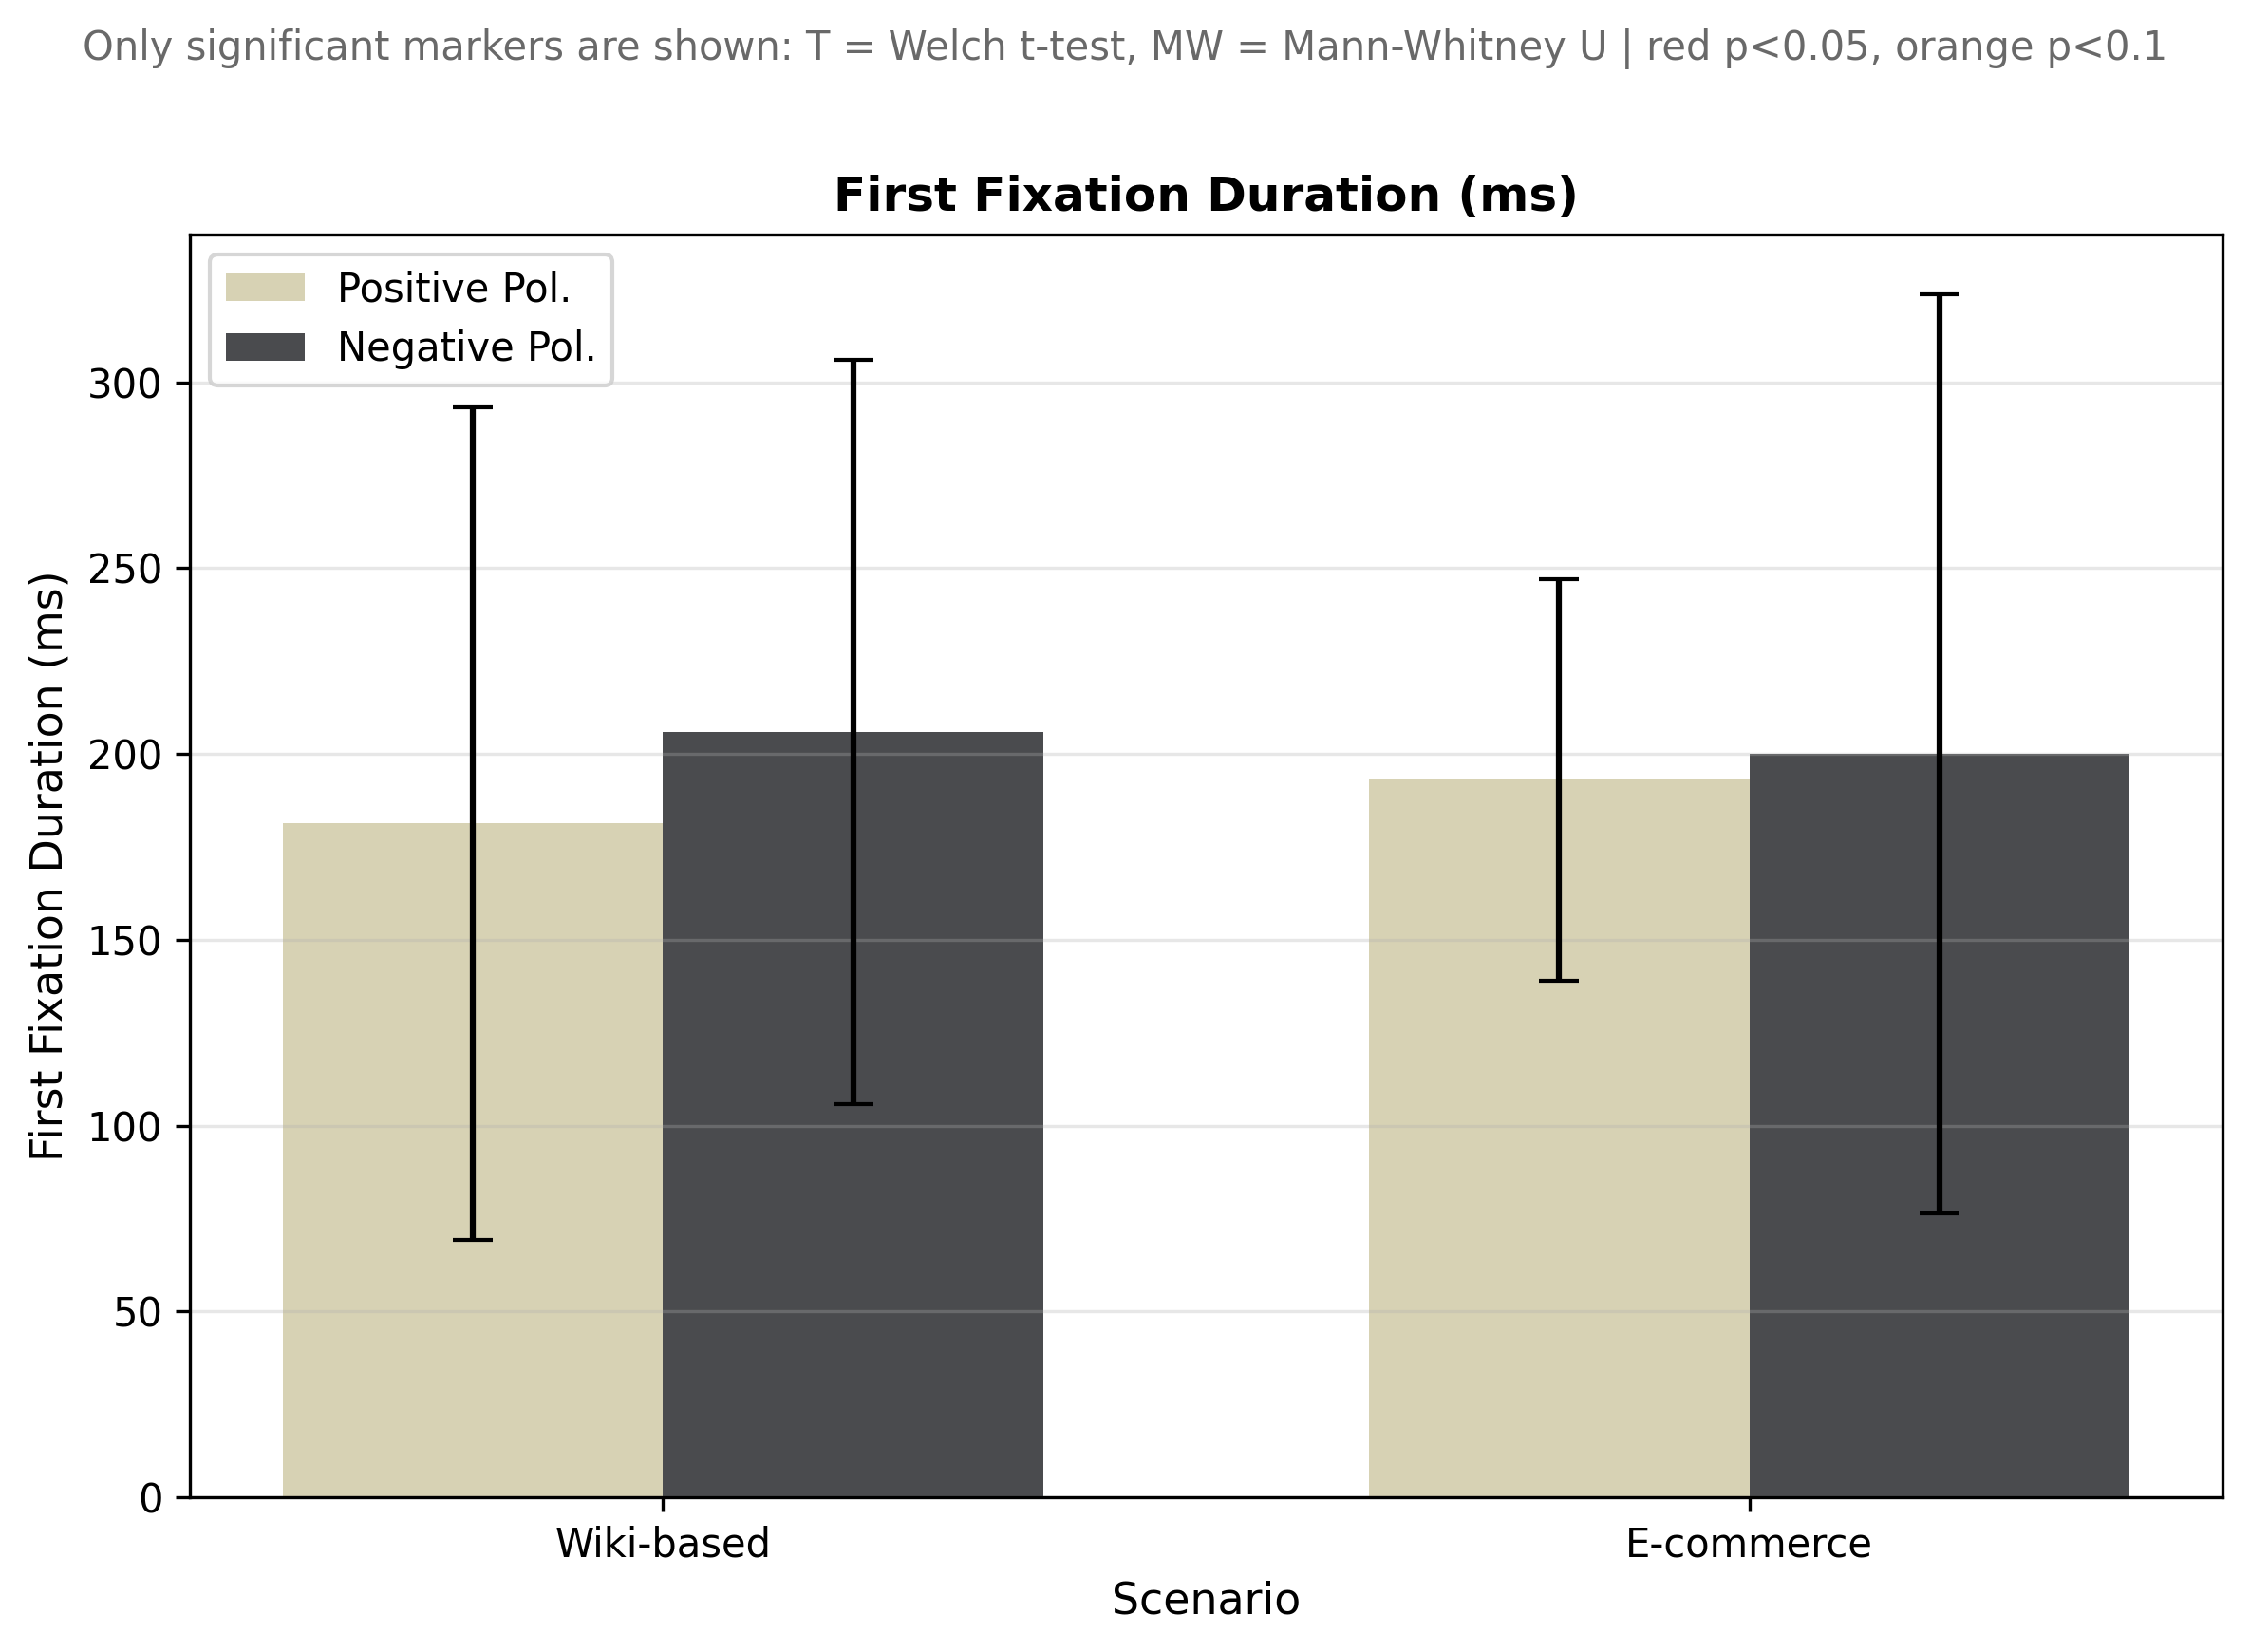
\includegraphics[width=0.8\textwidth]{figures/Duration_of_first_whole_fixation.png}
    \caption{Duration of First Fixation for each Display Polarity and TOI.}
    \label{fig:dfff_boxplot}
\end{figure}
The statistical analysis in this case shows how none of the TOIS follows a normal distribution, as shown in table
\ref{tab:dfff_stats} resulting in the Mann-Whitney U test where none of the TOIS is significant, see figure \ref{fig:dfff_boxplot}.
\begin{table}[H]
    \centering
    \small
    \setlength{\tabcolsep}{4pt}
    \caption{Statistics of Duration of First Fixation}
    \label{tab:dfff_stats}
    \resizebox{0.98\linewidth}{!}{
    \begin{tabular}{|c|c|c|c|c|}
        \hline
        \textbf{TOI} & \textbf{W\textsubscript{PP}} & \textbf{W\textsubscript{NP}} & \textbf{T-Student} & \textbf{Mann-Whitney} \\ \hline
        Wiki-Based & \textbf{\color{red}0.0001} & \textbf{\color{red}0.0005} & - & 0.3224 \\ \hline
        E-Commerce & \textbf{\color{red}0.0048} & \textbf{\color{red}0.0000} & - & 0.5434 \\ \hline
        Entire Exp. & \textbf{\color{red}0.0046} & \textbf{\color{red}0.0002} & - & 0.3005 \\ \hline
    \end{tabular}
    }
\end{table}

\subsection{Average Duration of Fixations}
The average duration of fixations seems to be higher in positive polarity in every single TOI, as shown in table
\ref{tab:adf_basic_stats}. This difference is more steep in the Wiki-Based scene.
\begin{table}[H]
    \centering
    \small
    \setlength{\tabcolsep}{4pt}
    \renewcommand{\arraystretch}{1.3}
    \caption{Results of Average Duration of Fixations}
    \label{tab:adf_basic_stats}

    \resizebox{0.98\linewidth}{!}{
    \begin{tabular}{|c|c|c|c|c|c|}
        \hline
        \textbf{Display Polarity} & \textbf{TOI} & \shortstack{\textbf{Min.} \\ \textbf{(ms)}} & \shortstack{\textbf{Mean} \\ \textbf{(ms)}} & \shortstack{\textbf{Std.} \\ \textbf{Deviation} \\ \textbf{(ms)}} & \shortstack{\textbf{Max.} \\ \textbf{(ms)}} \\ \hline
        

        \multirow{3}{*}{Positive Polarity} & \textbf{Wiki-based} & 234 & 329.29 & 79.39 & 537 \\ \cline{2-6}
         & \textbf{E-Commerce} & 236 & 318.41 & 63.58 & 457 \\ \cline{2-6}
         & \textbf{Entire Exp.} & 288 & 358.88 & 43.08 & 451 \\ \hline
        

        \multirow{3}{*}{Negative Polarity} & \textbf{Wiki-based} & 202 & 287.53 & 57.97 & 441 \\ \cline{2-6}
         & \textbf{E-Commerce} & 193 & 272.19 & 58.81 & 407 \\ \cline{2-6}
         & \textbf{Entire Exp.} & 262 & 336.18 & 46.65 & 436 \\ \hline
    \end{tabular}
    }
\end{table}
Regarding the statistical analysis, only a relevant result exists for the E-Commerce scene with the p-value of 0.0514 
being pretty close to the significance level.
\begin{figure}[H]
    \centering
    \includegraphics[width=0.8\textwidth]{figures/Average_Duration_of_whole_fixations.png}
    \caption{Average Duration of Fixations for each Display Polarity and TOI.}
    \label{fig:adf_boxplot}
\end{figure}
\begin{table}[H]
    \centering
    \small
    \setlength{\tabcolsep}{4pt}
    \caption{Statistics of Average Duration of Fixations}
    \label{tab:adf_stats}
    \resizebox{0.98\linewidth}{!}{
    \begin{tabular}{|c|c|c|c|c|}
        \hline
        \textbf{TOI} & \textbf{W\textsubscript{PP}} & \textbf{W\textsubscript{NP}} & \textbf{T-Student} & \textbf{Mann-Whitney} \\ \hline
        Wiki-Based & \textbf{\color{red}0.0365} & 0.2901 & - & 0.1528 \\ \hline
        E-Commerce & \textbf{\color{red}0.0200} & 0.4693 & - & \textbf{\color{orange}0.0514} \\ \hline
        Entire Exp. & 0.6286 & 0.8766 & 0.1624 & - \\ \hline
    \end{tabular}
    }
\end{table}

\subsection{Average Peak Velocity}
The average peak velocity is higher in negative polarity for every TOI as seen in table \ref{tab:apv_basic_stats}. However, 
It is only relevant in the entire recording with a p-value of 0.0871 proven in table \ref{tab:apv_stats} and figure \ref{fig:aspv_boxplot}
\begin{table}[H]
    \centering
    \small
    \setlength{\tabcolsep}{4pt}
    \renewcommand{\arraystretch}{1.3}
    \caption{Results of Average Peak Velocity}
    \label{tab:apv_basic_stats}

    \resizebox{0.98\linewidth}{!}{
    \begin{tabular}{|c|c|c|c|c|c|}
        \hline
        \textbf{Display Polarity} & \textbf{TOI} & \shortstack{\textbf{Min.} \\ \textbf{(º/s)}} & \shortstack{\textbf{Mean} \\ \textbf{(º/s)}} & \shortstack{\textbf{Std.} \\ \textbf{Deviation} \\ \textbf{(º/s)}} & \shortstack{\textbf{Max.} \\ \textbf{(º/s)}} \\ \hline
        

        \multirow{3}{*}{Positive Polarity} & \textbf{Wiki-based} & 89.13 & 107.76 & 15.84 & 148.82 \\ \cline{2-6}
         & \textbf{E-Commerce} & 77.19 & 102.25 & 24.92 & 189.92 \\ \cline{2-6}
         & \textbf{Entire Exp.} & 91.69 & 106.49 & 7.09 & 119.99 \\ \hline
        

        \multirow{3}{*}{Negative Polarity} & \textbf{Wiki-based} & 79.57 & 118.72 & 29.61 & 216.31 \\ \cline{2-6}
         & \textbf{E-Commerce} & 76.66 & 104.02 & 16.63 & 133.35 \\ \cline{2-6}
         & \textbf{Entire Exp.} & 88.48 & 112.61 & 11.79 & 135.44 \\ \hline
    \end{tabular}
    }
\end{table}
\begin{figure}[H]
    \centering
    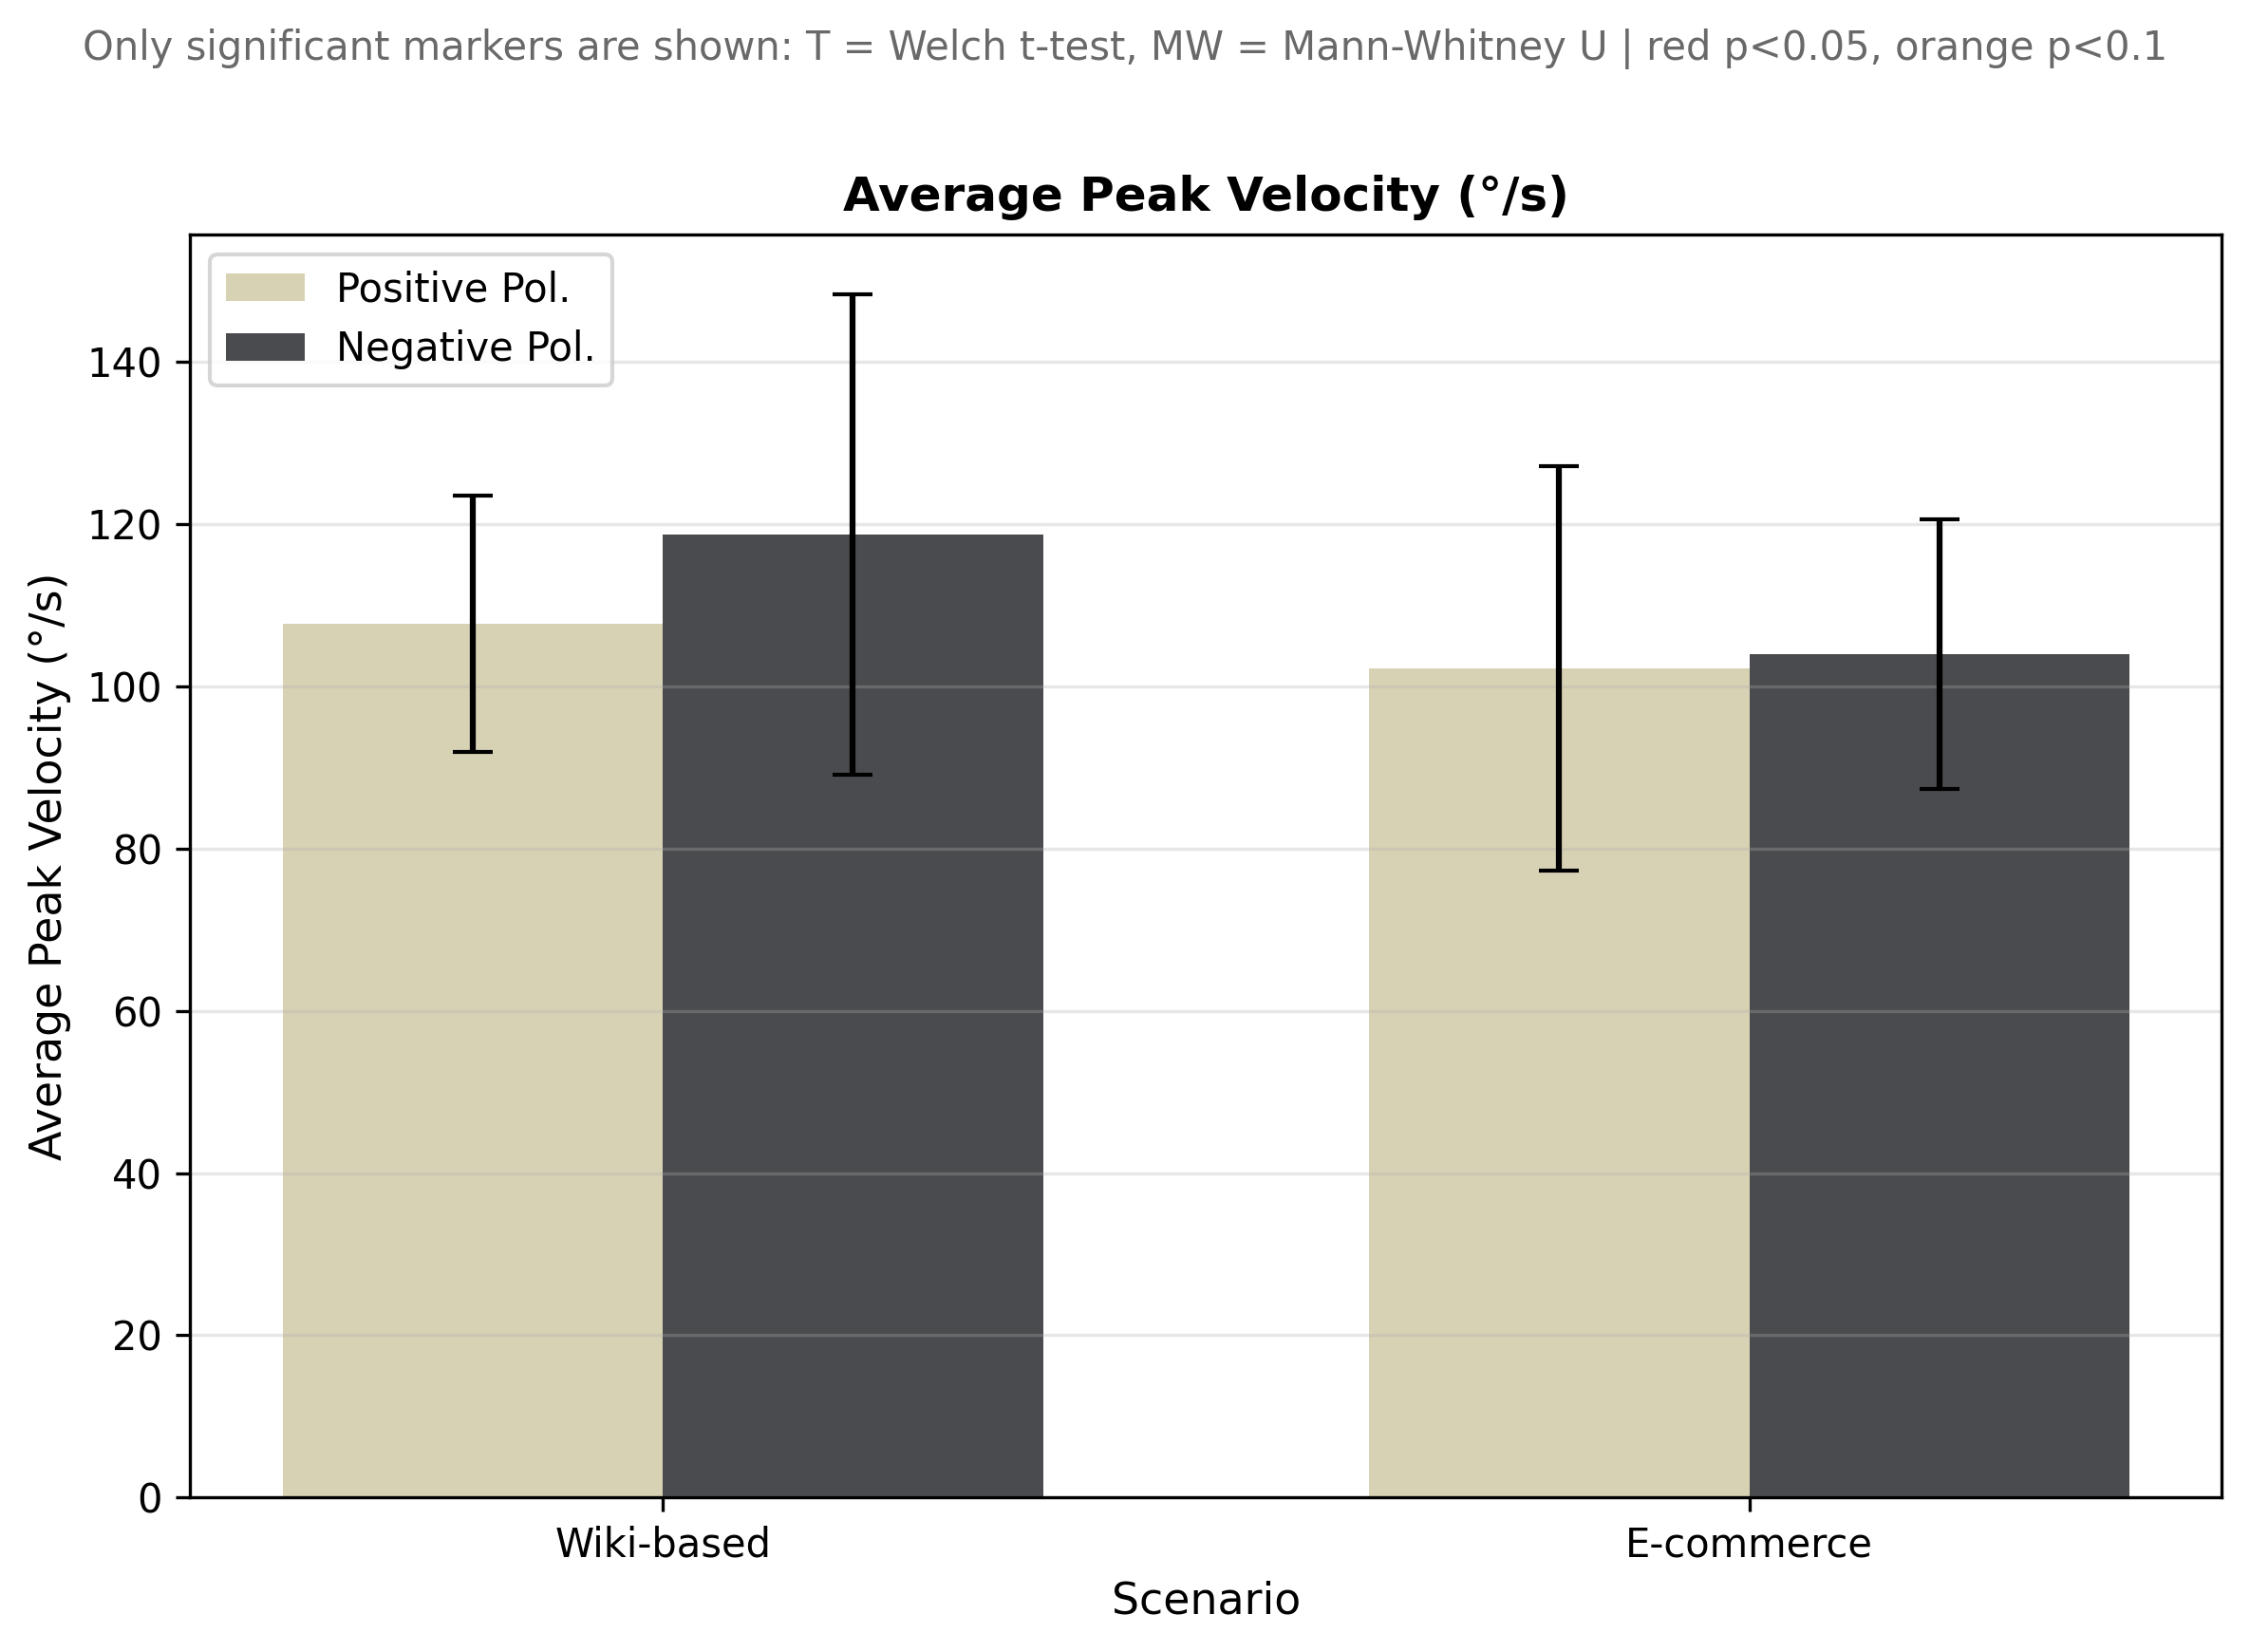
\includegraphics[width=0.8\textwidth]{figures/Average_peak_velocity_of_saccades.png}
    \caption{Average Saccade Peak Velocity for each Display Polarity and TOI.}
    \label{fig:aspv_boxplot}
\end{figure}
\begin{table}[H]
    \centering
    \small
    \setlength{\tabcolsep}{4pt}
    \caption{Statistics of Average Peak Velocity}
    \label{tab:apv_stats}
    \resizebox{0.98\linewidth}{!}{
    \begin{tabular}{|c|c|c|c|c|}
        \hline
        \textbf{TOI} & \textbf{W\textsubscript{PP}} & \textbf{W\textsubscript{NP}} & \textbf{T-Student} & \textbf{Mann-Whitney} \\ \hline
        Wiki-Based & \textbf{\color{red}0.0371} & \textbf{\color{red}0.0030} & - & 0.2557 \\ \hline
        E-Commerce & \textbf{\color{red}0.0001} & 0.5860 & - & 0.3892 \\ \hline
        Entire Exp. & 0.3574 & 0.9985 & \textbf{\color{orange}0.0871} & - \\ \hline
    \end{tabular}
    }
\end{table}

\subsection{Average Saccade Amplitude}
The results of table \ref{tab:asa_basic_stats} show a pretty even mean distribution along polarities making no evident
differences. This can be further seen in figure \ref{fig:asa_boxplot} and table \ref{tab:asa_stats} where none of the statistics
is close to be significant.
\begin{table}[H]
    \centering
    \small
    \setlength{\tabcolsep}{4pt}
    \renewcommand{\arraystretch}{1.3}
    \caption{Results of Average Saccade Amplitude}
    \label{tab:asa_basic_stats}

    \resizebox{0.98\linewidth}{!}{
    \begin{tabular}{|c|c|c|c|c|c|}
        \hline
        \textbf{Display Polarity} & \textbf{TOI} & \shortstack{\textbf{Min.} \\ \textbf{(º)}} & \shortstack{\textbf{Mean} \\ \textbf{(º)}} & \shortstack{\textbf{Std.} \\ \textbf{Deviation} \\ \textbf{(º)}} & \shortstack{\textbf{Max.} \\ \textbf{(º)}} \\ \hline
        

        \multirow{3}{*}{Positive Polarity} & \textbf{Wiki-based} & 2.22 & 2.97 & 0.48 & 3.87 \\ \cline{2-6}
         & \textbf{E-Commerce} & 1.92 & 2.95 & 0.70 & 5.15 \\ \cline{2-6}
         & \textbf{Entire Exp.} & 2.39 & 3.12 & 0.36 & 3.70 \\ \hline
        

        \multirow{3}{*}{Negative Polarity} & \textbf{Wiki-based} & 2.26 & 3.26 & 0.69 & 5.30 \\ \cline{2-6}
         & \textbf{E-Commerce} & 2.14 & 2.98 & 0.50 & 4.06 \\ \cline{2-6}
         & \textbf{Entire Exp.} & 2.63 & 3.31 & 0.39 & 4.10 \\ \hline
    \end{tabular}
    }
\end{table}
\begin{figure}[H]
    \centering
    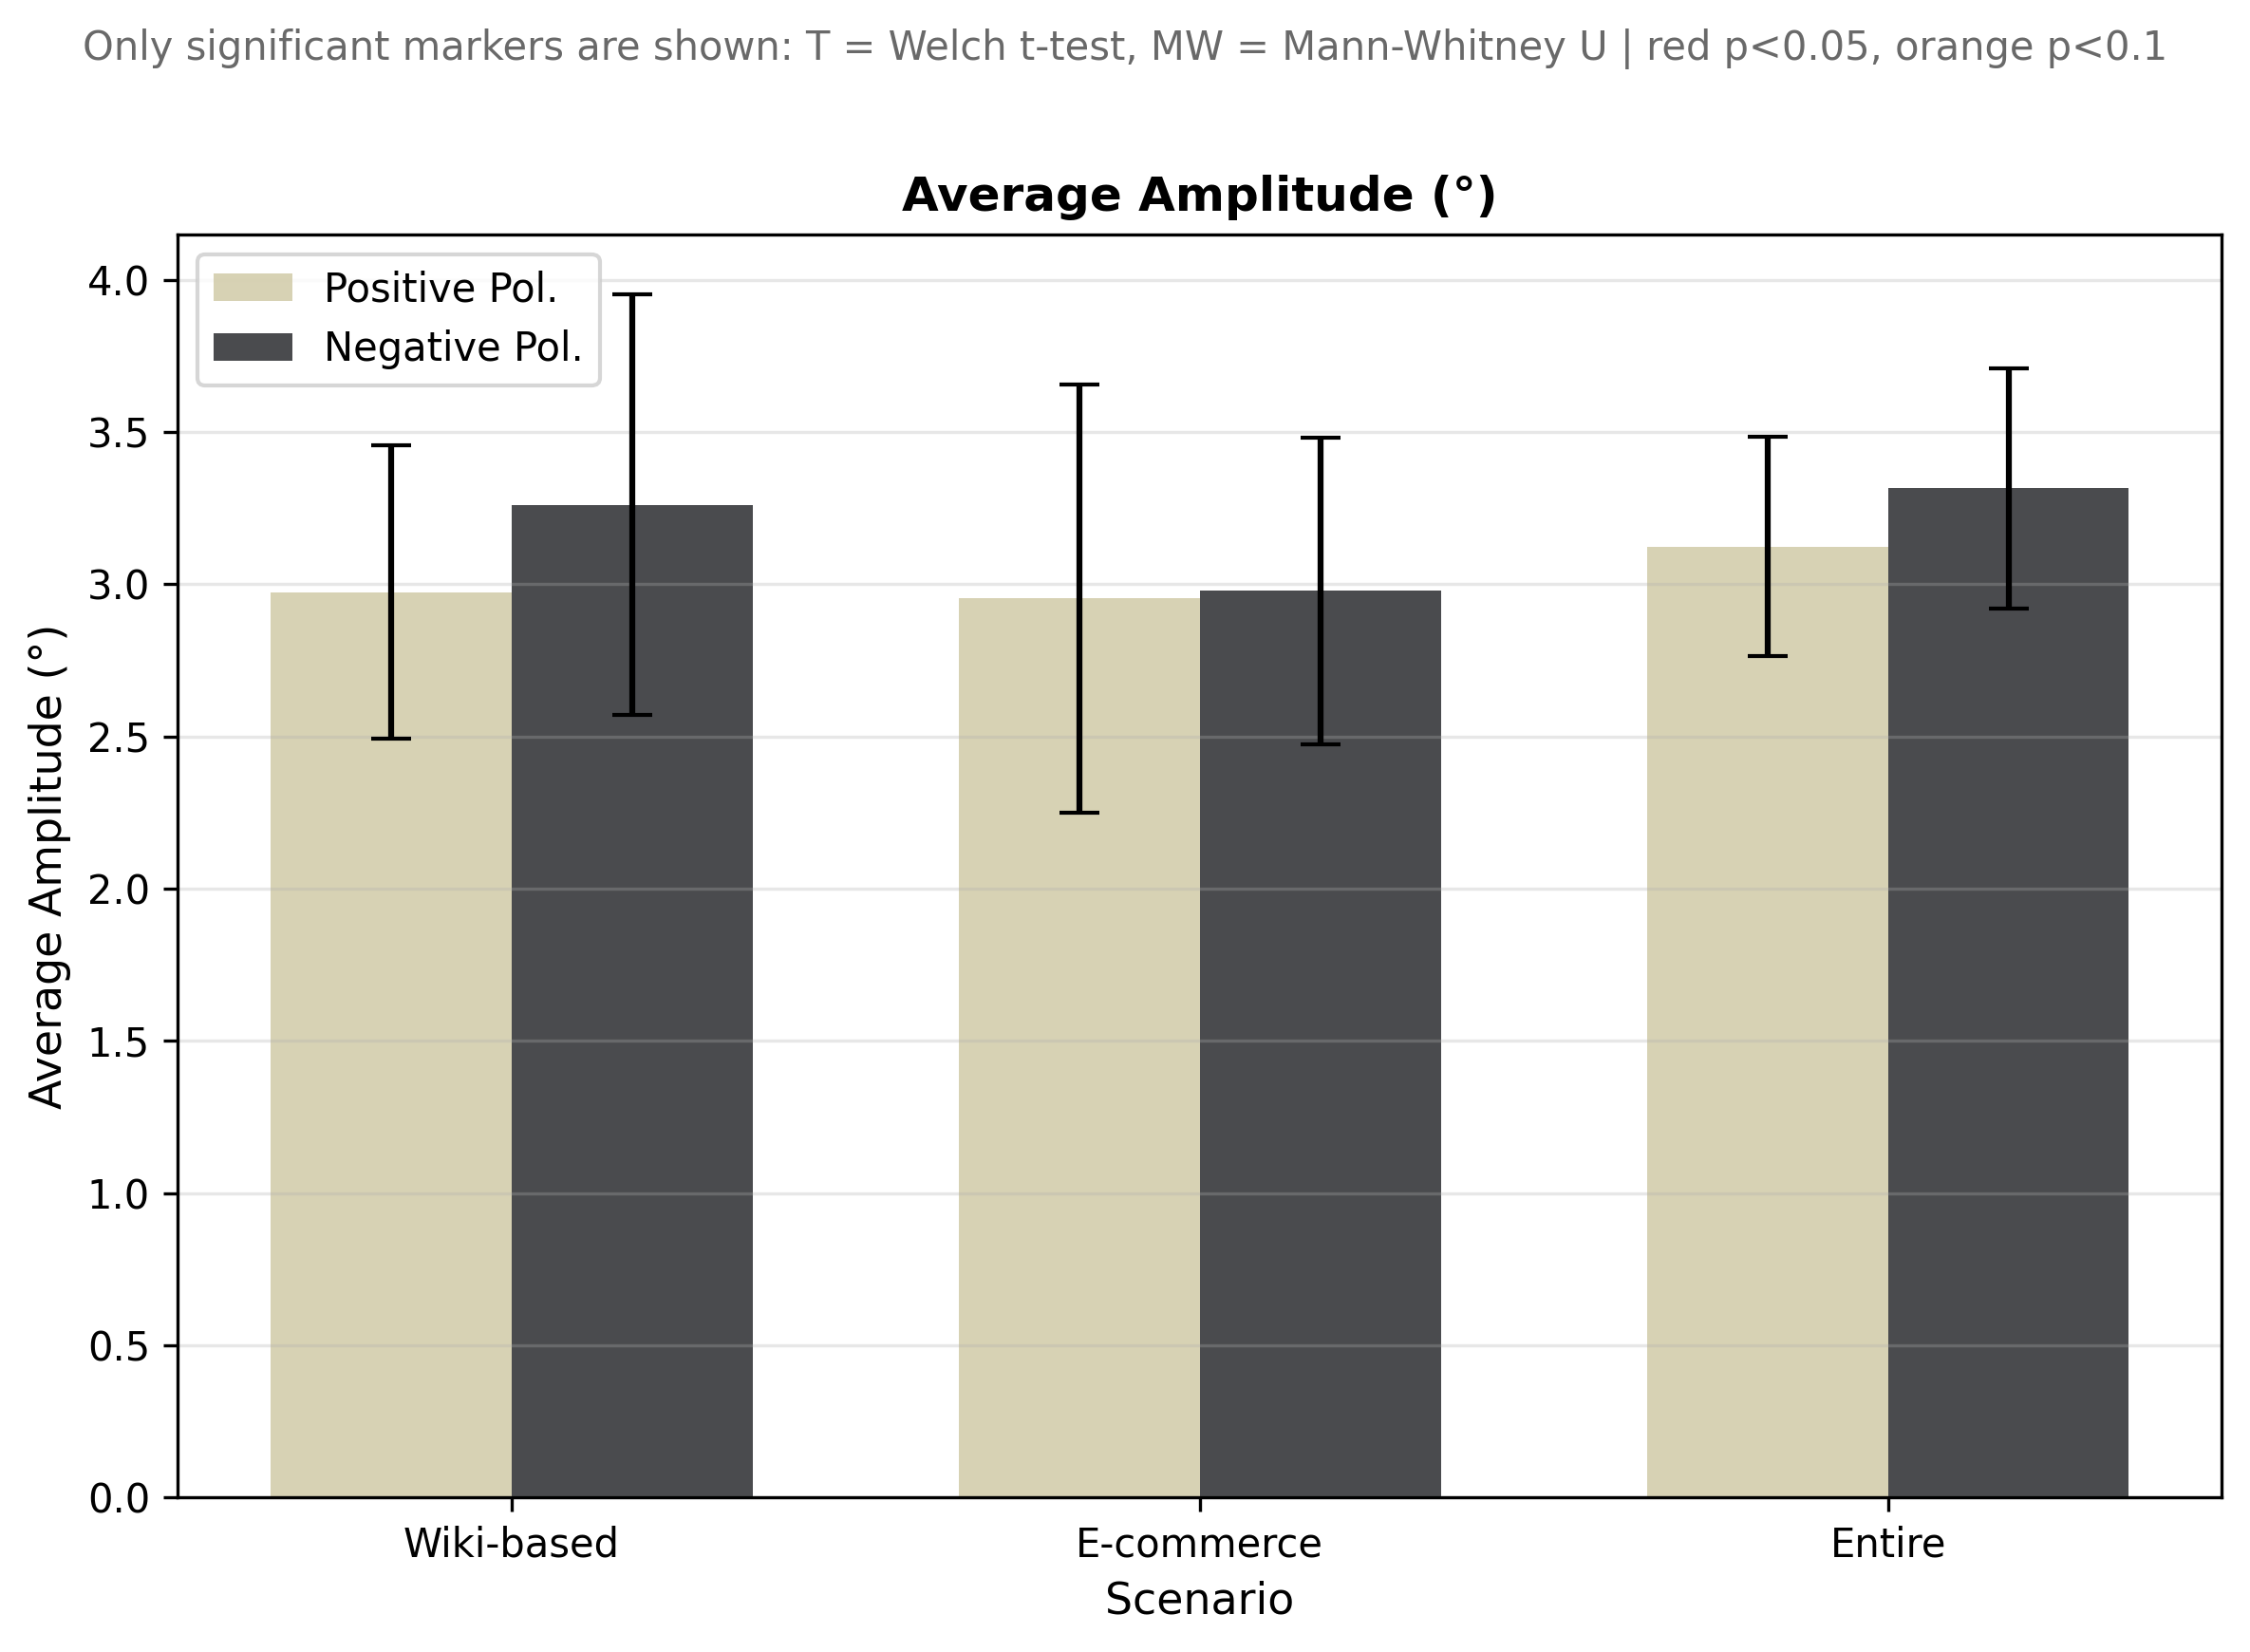
\includegraphics[width=0.8\textwidth]{figures/Average_amplitude_of_saccades.png}
    \caption{Average Saccade Amplitude for each Display Polarity and TOI.}
    \label{fig:asa_boxplot}
\end{figure}
\begin{table}[H]
    \centering
    \small
    \setlength{\tabcolsep}{4pt}
    \caption{Statistics of Average Saccade Amplitude}
    \label{tab:asa_stats}
    \resizebox{0.98\linewidth}{!}{
    \begin{tabular}{|c|c|c|c|c|}
        \hline
        \textbf{TOI} & \textbf{W\textsubscript{PP}} & \textbf{W\textsubscript{NP}} & \textbf{T-Student} & \textbf{Mann-Whitney} \\ \hline
        Wiki-Based & 0.6837 & \textbf{\color{orange}0.0758} & 0.1833 & - \\ \hline
        E-Commerce & \textbf{\color{red}0.0153} & 0.6737 & - & 0.6297 \\ \hline
        Entire Exp. & \textbf{\color{orange}0.0984} & 0.9634 & 0.1620 & - \\ \hline
    \end{tabular}
    }
\end{table}
\subsection{Amplitude of First Saccade}
The amplitude of the first saccade behaved simmilarly to the average saccade amplitude with a pretty even mean distribution.
Followd with a big standard deviation shown in table \ref{tab:afas_basic_stats}. This can be further seen in figure \ref{fig:afas_boxplot} and table \ref{tab:afas_stats}
 this also leads to no significant nor meaningful results in the statistics table \ref{tab:afas_stats}
\begin{table}[H]
    \centering
    \small
    \setlength{\tabcolsep}{4pt}
    \renewcommand{\arraystretch}{1.3}
    \caption{Results of Amplitude of First Saccade}
    \label{tab:afas_basic_stats}

    \resizebox{0.98\linewidth}{!}{
    \begin{tabular}{|c|c|c|c|c|c|}
        \hline
        \textbf{Display Polarity} & \textbf{TOI} & \shortstack{\textbf{Min.} \\ \textbf{(º)}} & \shortstack{\textbf{Mean} \\ \textbf{(º)}} & \shortstack{\textbf{Std.} \\ \textbf{Deviation} \\ \textbf{(º)}} & \shortstack{\textbf{Max.} \\ \textbf{(º)}} \\ \hline
        

        \multirow{3}{*}{Positive Polarity} & \textbf{Wiki-based} & 1.59 & 9.06 & 3.93 & 17.71 \\ \cline{2-6}
         & \textbf{E-Commerce} & 0.56 & 5.35 & 3.29 & 13.00 \\ \cline{2-6}
         & \textbf{Entire Exp.} & 1.07 & 5.18 & 3.97 & 17.74 \\ \hline
        

        \multirow{3}{*}{Negative Polarity} & \textbf{Wiki-based} & 2.03 & 8.74 & 3.79 & 14.09 \\ \cline{2-6}
         & \textbf{E-Commerce} & 0.56 & 4.70 & 3.39 & 14.86 \\ \cline{2-6}
         & \textbf{Entire Exp.} & 0.59 & 6.46 & 4.57 & 17.47 \\ \hline
    \end{tabular}
    }
\end{table}
\begin{figure}[H]
    \centering
    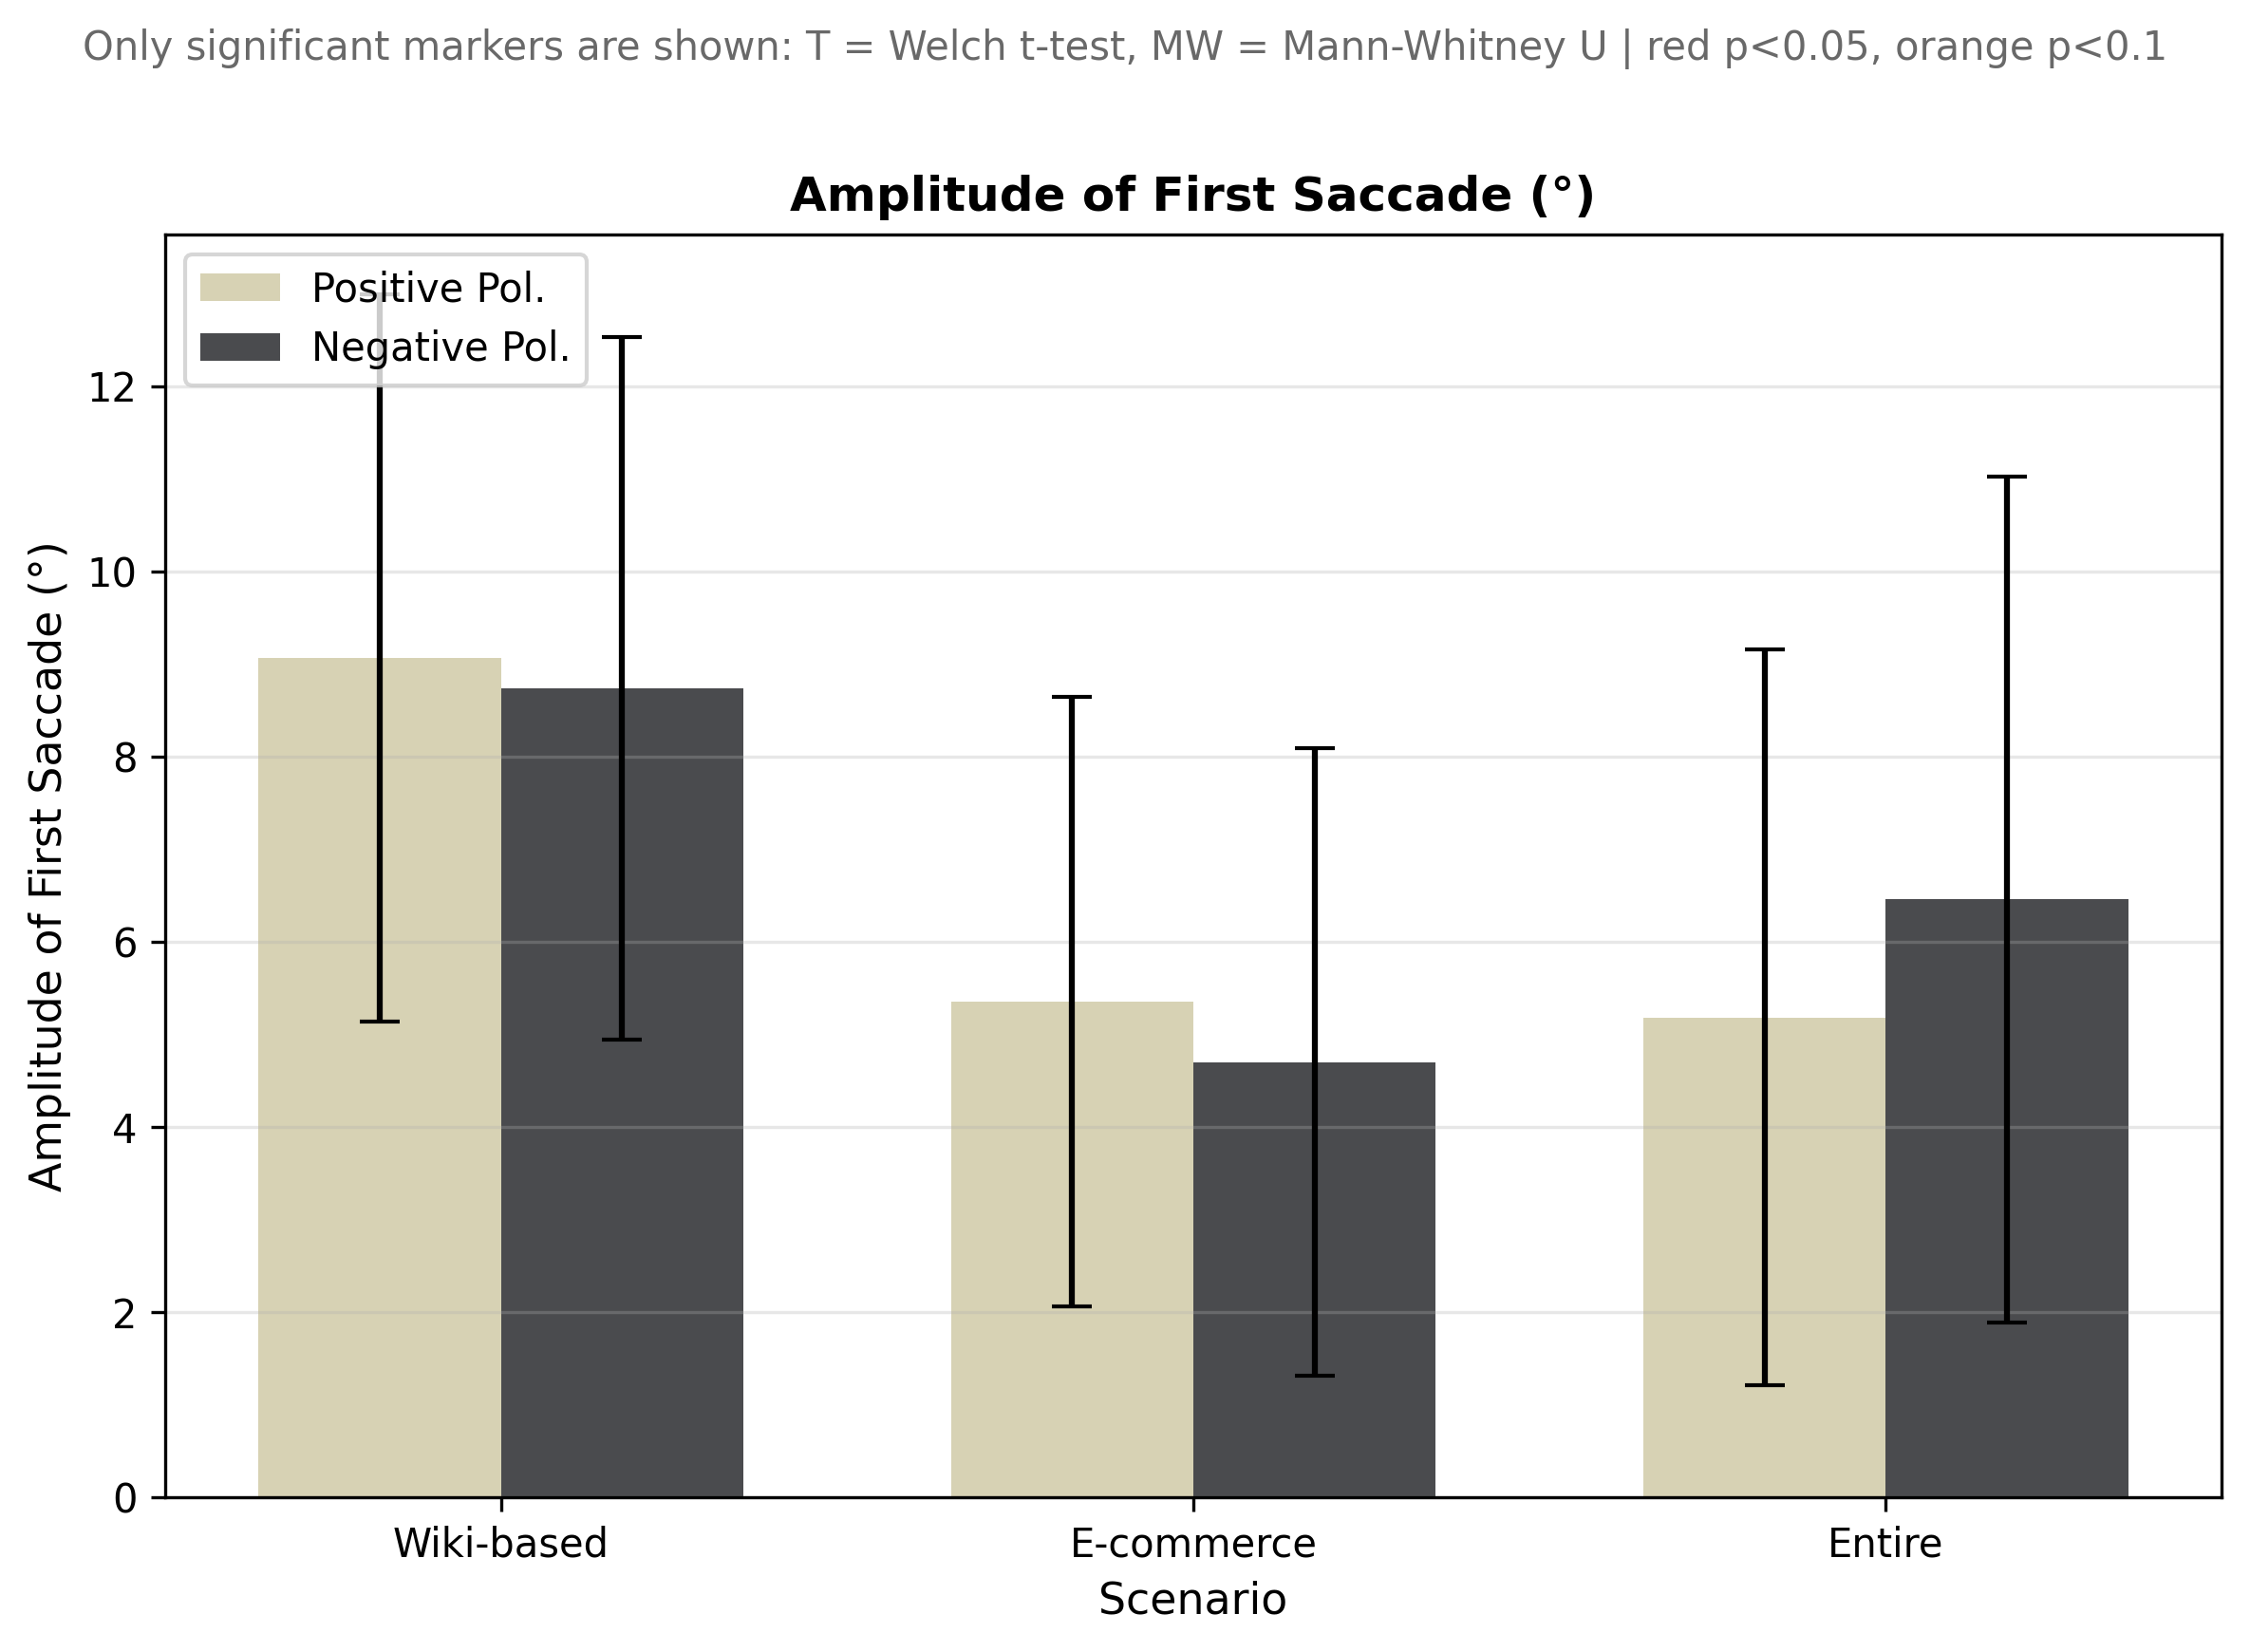
\includegraphics[width=0.8\textwidth]{figures/Amplitude_of_first_saccade.png}
    \caption{Amplitude of First Saccade for each Display Polarity and TOI.}
    \label{fig:afas_boxplot}
\end{figure}
\begin{table}[H]
    \centering
    \small
    \setlength{\tabcolsep}{4pt}
    \caption{Statistics of Amplitude of First Saccade}
    \label{tab:afas_stats}
    \resizebox{0.98\linewidth}{!}{
    \begin{tabular}{|c|c|c|c|c|}
        \hline
        \textbf{TOI} & \textbf{W\textsubscript{PP}} & \textbf{W\textsubscript{NP}} & \textbf{T-Student} & \textbf{Mann-Whitney} \\ \hline
        Wiki-Based & 0.5576 & 0.2155 & 0.8151 & - \\ \hline
        E-Commerce & 0.3231 & \textbf{\color{red}0.0159} & - & 0.5018 \\ \hline
        Entire Exp. & \textbf{\color{red}0.0030} & 0.1831 & - & 0.5353 \\ \hline
    \end{tabular}
    }
\end{table}
\subsection{Number of Saccades}
Lastly, all 3 scenes had a higher mean number of saccades in positive polarity than in negative polarity clearly shown
in table \ref{tab:ns_basic_stats}. 
\begin{table}[H]
    \centering
    \small
    \setlength{\tabcolsep}{4pt}
    \renewcommand{\arraystretch}{1.3}
    \caption{Results of Number of Saccades}
    \label{tab:ns_basic_stats}

    \resizebox{0.98\linewidth}{!}{
    \begin{tabular}{|c|c|c|c|c|c|}
        \hline
        \textbf{Display Polarity} & \textbf{TOI} & \shortstack{\textbf{Min.}} & \shortstack{\textbf{Mean}} & \shortstack{\textbf{Std.} \\ \textbf{Deviation}} & \shortstack{\textbf{Max.}} \\ \hline
        

        \multirow{3}{*}{Positive Polarity} & \textbf{Wiki-based} & 59 & 151.29 & 47.86 & 270 \\ \cline{2-6}
         & \textbf{E-Commerce} & 34 & 184.18 & 83.67 & 305 \\ \cline{2-6}
         & \textbf{Entire Exp.} & 509 & 870.06 & 188.81 & 1122 \\ \hline
        

        \multirow{3}{*}{Negative Polarity} & \textbf{Wiki-based} & 13 & 134.41 & 50.24 & 199 \\ \cline{2-6}
         & \textbf{E-Commerce} & 29 & 171.47 & 59.10 & 241 \\ \cline{2-6}
         & \textbf{Entire Exp.} & 344 & 746.41 & 166.22 & 1004 \\ \hline
    \end{tabular}
    }
\end{table}
There's only a relevant results regardin the whole recording with a p-value of 0.0582 in the t-student test. It is not enough to be 
considered relevant but gets close enough to be considered relevant. This can be further seen in figure \ref{fig:ns_boxplot} and table \ref{tab:ns_stats}.
\begin{figure}[H]
    \centering
    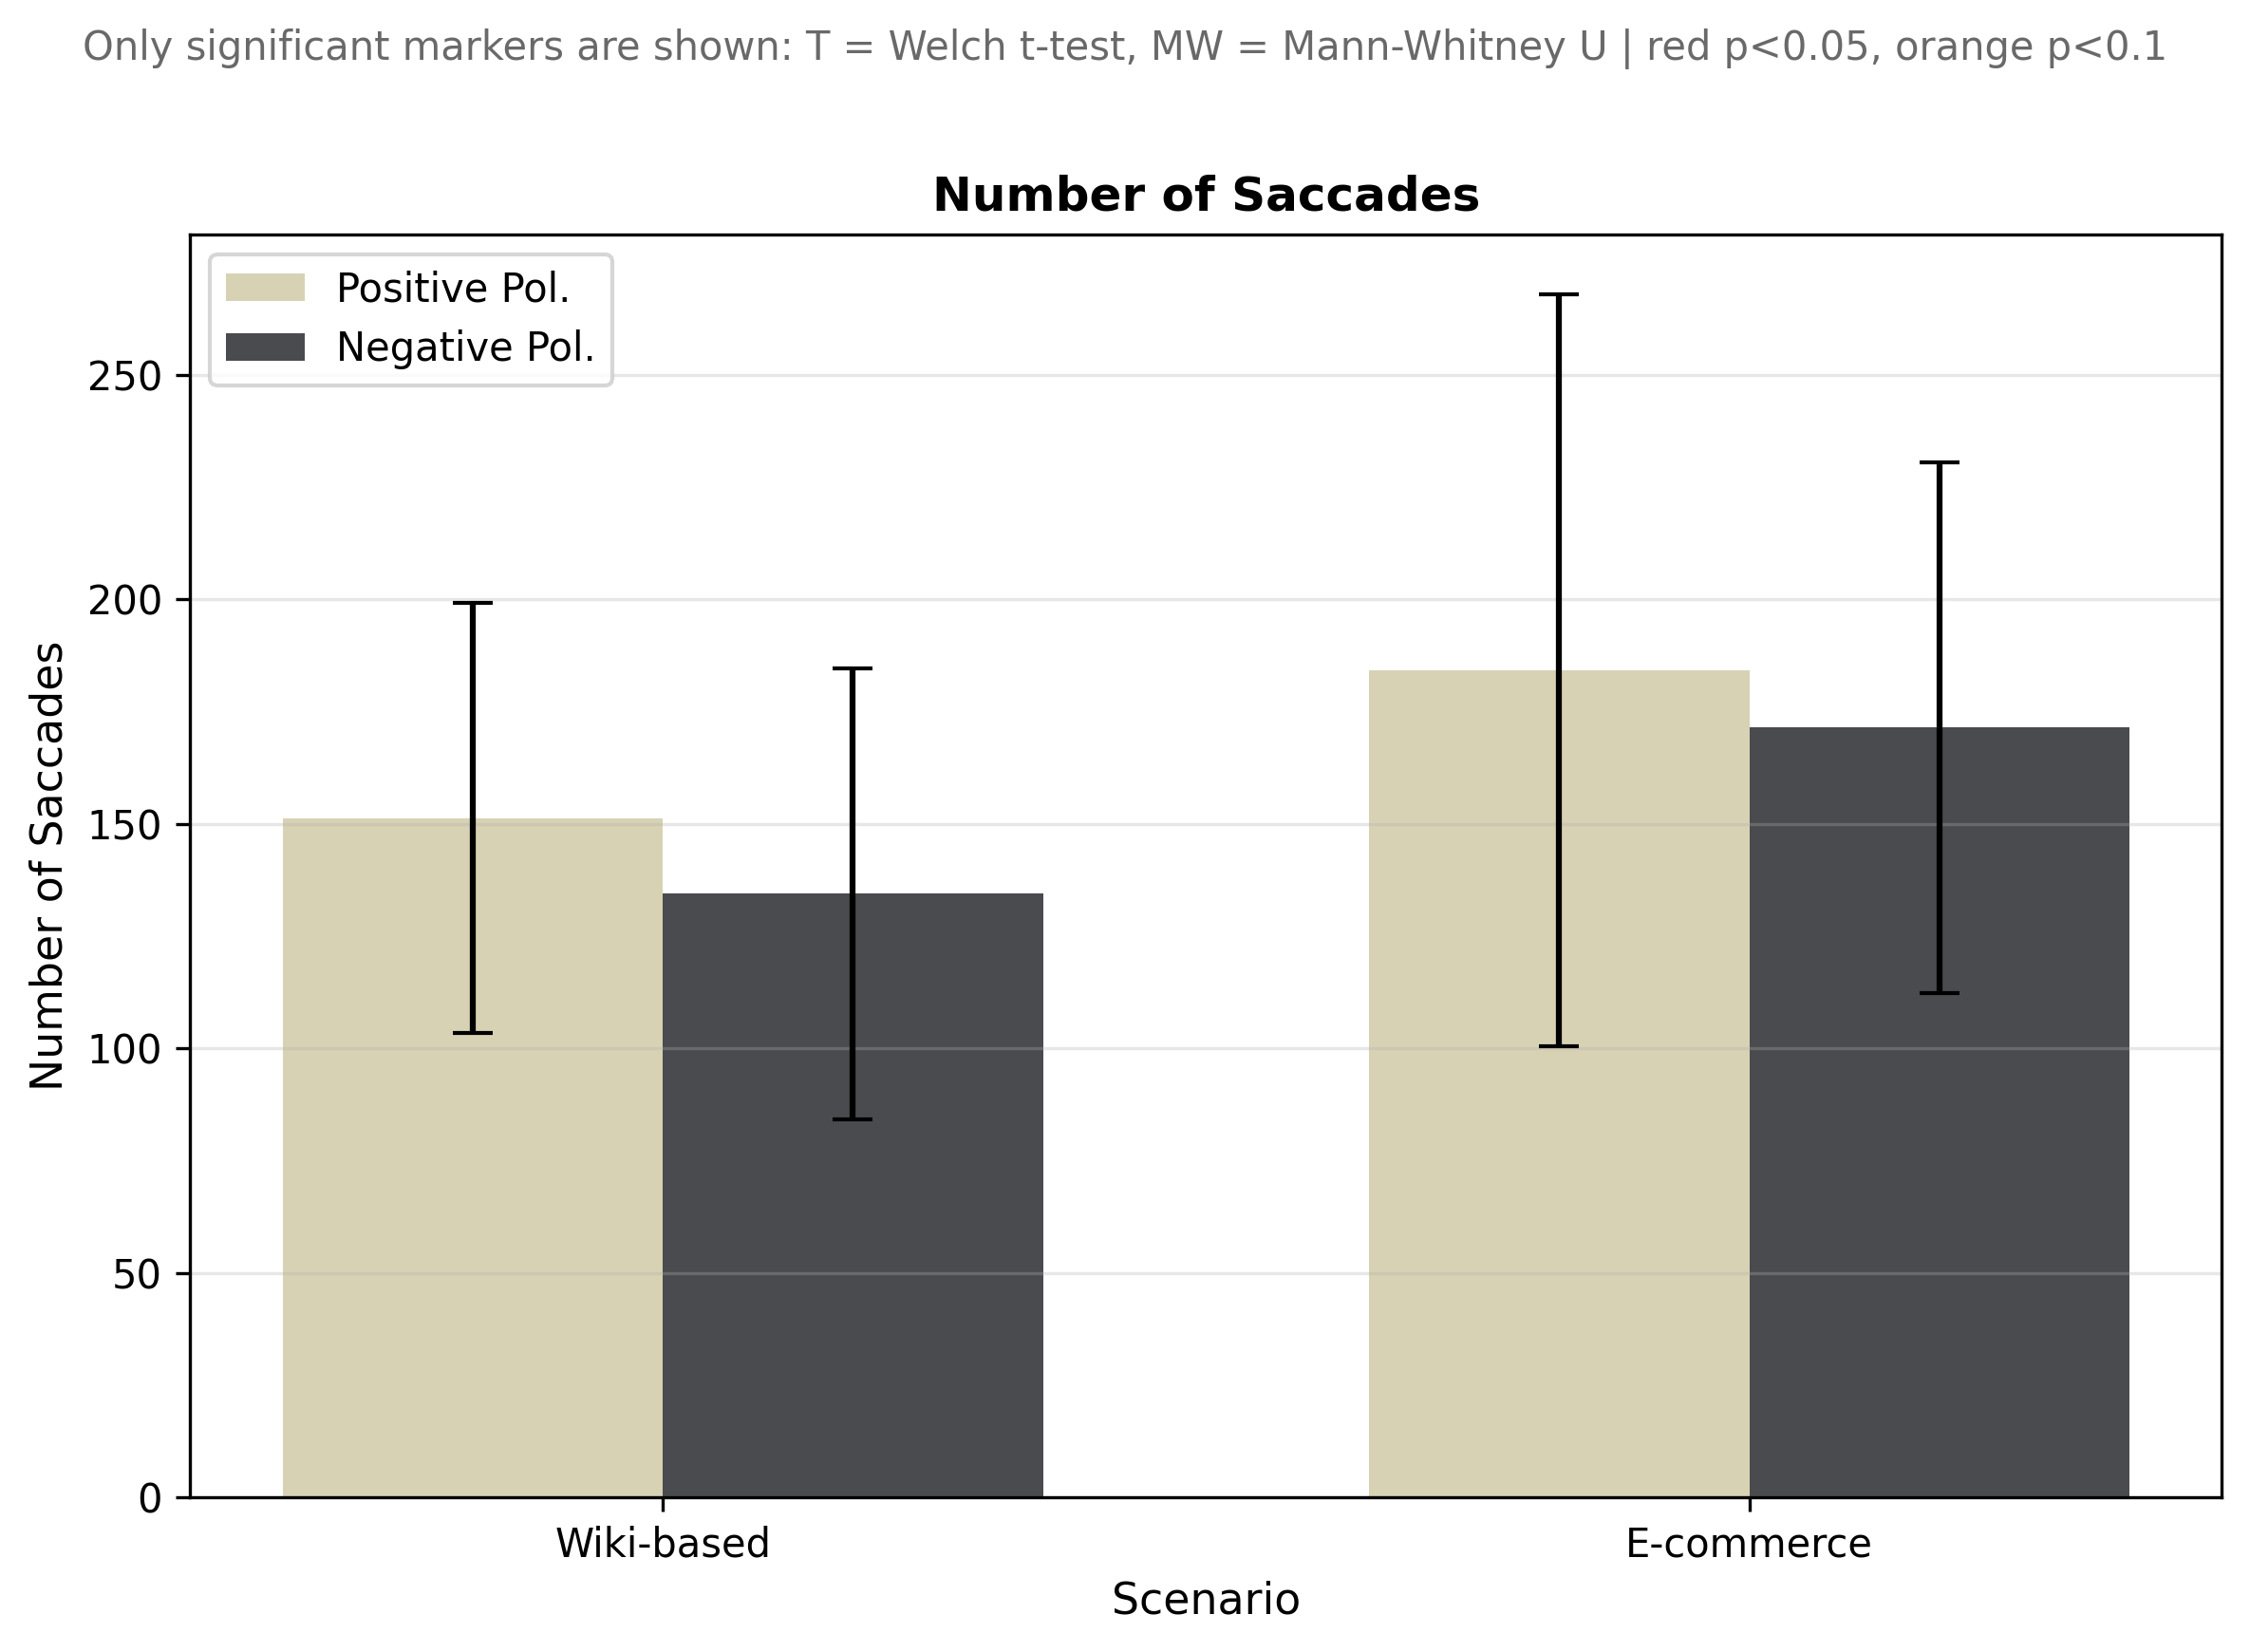
\includegraphics[width=0.8\textwidth]{figures/Number_of_saccades.png}
    \caption{Number of Saccades for each Display Polarity and TOI.}
    \label{fig:ns_boxplot}
\end{figure}
\begin{table}[H]
    \centering
    \small
    \setlength{\tabcolsep}{4pt}
    \caption{Statistics of Number of Saccades}
    \label{tab:ns_stats}
    \resizebox{0.98\linewidth}{!}{
    \begin{tabular}{|c|c|c|c|c|}
        \hline
        \textbf{TOI} & \textbf{W\textsubscript{PP}} & \textbf{W\textsubscript{NP}} & \textbf{T-Student} & \textbf{Mann-Whitney} \\ \hline
        Wiki-Based & 0.9486 & 0.2609 & 0.3377 & - \\ \hline
        E-Commerce & 0.1768 & \textbf{\color{red}0.0185} & - & 0.3797 \\ \hline
        Entire Exp. & 0.1577 & 0.6058 & \textbf{\color{orange}0.0582} & - \\ \hline
    \end{tabular}
    }
\end{table}
\section{Questionnaire Results}
This section will provide an insight of the results obtained through the Google Forms
Questionnaire. The results will be shown along with an ID, this ID corresponds to
the first letter of the subsection name in the section \ref{sec:final_questionnaire} 
followed by the number of the question. For example, the first question of the Wiki-Based
Scene will be identified as W1, the second question of the E-Commerce Scene will be identified 
as E2 and so on.
\subsection{Reading Comprehension Questions}
\subsubsection{Wiki-Based}
Overall results seen in table \ref{tab:rcq_wiki_results} show that the percentage of correct answers 
is higher in negative polarity than in positive polarity in every question but in $W3$ where
the differences are pretty steep.
\begin{table}[H]
    \centering
    \small
    \setlength{\tabcolsep}{4pt}
    \renewcommand{\arraystretch}{1.3}
    \caption{Basic data per question of the Wiki-Based Scene}
    \label{tab:rcq_wiki_results}

    \resizebox{0.98\linewidth}{!}{
    \begin{tabular}{|c|c|c|c|c|}
        \hline
        \textbf{Question ID} & \textbf{Correct Answers} & \textbf{Wrong Answers} & \textbf{PP Correct(\%)} & \textbf{NP Correct(\%)} \\ \hline
        W1 & 15 & 19 & 29.41 & 58.82 \\ \hline
        W2 &  21 & 13 & 41.18 & 82.36\\ \hline
        W3 &  20 & 14 & 70.59 & 47.06\\ \hline
        W4 &  24 & 10 & 64.71 & 76.47 \\ \hline
    \end{tabular}
    }
\end{table}
\subsubsection{E-Commerce}
E-Commerce results in table \ref{tab:rcq_ecommerce_results} show a pretty even distribution of 
correct answers between both polarities. The question $E3$ is surprisingly a bit lower in 
negative polarity as this question was pretty simple.
\begin{table}[H]
    \centering
    \small
    \setlength{\tabcolsep}{4pt}
    \renewcommand{\arraystretch}{1.3}
    \caption{Basic data per question of the E-Commerce Scene}
    \label{tab:rcq_ecommerce_results}

    \resizebox{0.98\linewidth}{!}{
    \begin{tabular}{|c|c|c|c|c|}
        \hline
        \textbf{Question ID} & \textbf{Correct Answers} & \textbf{Wrong Answers} & \textbf{PP Correct(\%)} & \textbf{NP Correct(\%)} \\ \hline
        E1 & 34 & 0 & 100 & 100 \\ \hline
        E2 &  18 & 16 & 47.06 & 58.83 \\ \hline
        E3 &  28 & 6 & 88.24 & 76.47\\ \hline
        E4 &  21 & 13 & 64.71 & 58.82 \\ \hline
    \end{tabular}
    }
\end{table}
\subsection{Preference Questions}
The questionnaire is divided in two types of questions, categorical and numeric. The categorial questions are those
where the participant chooses from a non numeric list of options. For example, In question P1 the participant had to choose
between "Normal Vision" and "Corrected Vision". On the other hand, the numeric questions are those where 
the experimentee answers with a numerical value.
\subsubsection{Categorical Questions}
The experiment remained consistent not only in gender and age distribution as seen in chapter \ref{chap:methodology}
but also in the type of vision of the participants as shown in table \ref{tab:participants_vision}. This consistency 
results in a 53\% of participants with normal vision and a 47\% of participants with corrected vision in both polarities.
\begin{table}[H]
    \centering
    \caption{Type of vision of the participants (Question P1)}
    \label{tab:participants_vision}
    \begin{tabular}{|c|c|c|}
        \hline
        \textbf{Polarity} & \textbf{Normal Vision} & \textbf{Corrected Vision} \\ \hline
        Positive Polarity & 9 & 8 \\ \hline
        Negative Polarity & 9 & 8 \\ \hline
    \end{tabular}
\end{table}
The display polarity preference for both scenes shows a slight preference for white background with black text 
in the Wiki-Based scene as shown in table \ref{tab:wiki_preference}
\begin{table}[H]
    \centering
    \caption{Wiki-Based Scene Preference (Question P2)}
    \label{tab:wiki_preference}
    \begin{tabular}{|c|c|c|}
        \hline
        \textbf{Experiment Polarity} & \textbf{\shortstack{Positive Polarity\\Preferred}} & \textbf{\shortstack{Negative Polarity\\Preferred}} \\ \hline
        Positive Polarity & 11 & 6 \\ \hline
        Negative Polarity & 9 & 8 \\ \hline
    \end{tabular}
\end{table}
The trend in the E-Commerce scene is simmilar to the Wiki-Based scene having an increase for 
the positive polarity as seen in table \ref{tab:ecommerce_preference}.
\begin{table}[H]
    \centering
    \caption{E-Commerce Scene Preference (Question P3)}
    \label{tab:ecommerce_preference}
    \begin{tabular}{|c|c|c|}
        \hline
        \textbf{Experiment Polarity} & \textbf{\shortstack{Positive Polarity\\Preferred}} & \textbf{\shortstack{Negative Polarity\\Preferred}} \\ \hline
        Positive Polarity & 11 & 6 \\ \hline
        Negative Polarity & 12 & 5 \\ \hline
    \end{tabular}
\end{table}
\subsubsection{Numeric Questions}
Regardin the numeric questions, the results in table \ref{tab:numeric_descriptor} should be read along with the 
questions in chapter \ref{sec:final_questionnaire} to understand every question. Overall, the results appeared 
to be pretty even between polarities.
\begin{table}[H]
    \centering
    \small
    \setlength{\tabcolsep}{4pt}
    \renewcommand{\arraystretch}{1.3}
    \caption{Numeric Preference Descriptive Statistics}
    \label{tab:numeric_descriptor}

    \resizebox{0.98\linewidth}{!}{
    \begin{tabular}{|c|c|c|c|c|c|}
        \hline
        \textbf{Question ID} & \textbf{Display Polarity} & \textbf{Min.} & \textbf{Mean} & \textbf{Std. Deviation} & \textbf{Max.} \\ \hline
           \multirow{2}{*}{P4} & Positive & 1 & 3.29 & 1.36 & 5 \\ \cline{2-6}
            & Negative & 1 & 3.65 & 1.41 & 5 \\ \hline
           \multirow{2}{*}{P5} & Positive & 1 & 2.82 & 1.51 & 5 \\ \cline{2-6}
            & Negative & 1 & 2.76 & 1.48 & 5 \\ \hline
           \multirow{2}{*}{P6} & Positive & 3 & 4.00 & 0.71 & 5 \\ \cline{2-6}
            & Negative & 2 & 4.24 & 0.90 & 5 \\ \hline
           \multirow{2}{*}{P7} & Positive & 2 & 3.71 & 0.85 & 5 \\ \cline{2-6}
            & Negative & 2 & 3.65 & 0.79 & 5 \\ \hline
           \multirow{2}{*}{P8} & Positive & 2 & 3.76 & 0.75 & 5 \\ \cline{2-6}
            & Negative & 2 & 3.88 & 0.93 & 5 \\ \hline
           \multirow{2}{*}{P9} & Positive & 3 & 4.00 & 0.87 & 5 \\ \cline{2-6}
            & Negative & 2 & 3.59 & 0.87 & 5 \\ \hline
           \multirow{2}{*}{P10} & Positive & 2 & 3.47 & 0.94 & 5 \\ \cline{2-6}
            & Negative & 2 & 3.47 & 1.07 & 5 \\ \hline
           \multirow{2}{*}{P11} & Positive & 1 & 3.41 & 1.37 & 5 \\ \cline{2-6}
            & Negative & 1 & 3.35 & 1.00 & 5 \\ \hline
           \multirow{2}{*}{P12} & Positive & 3 & 4.12 & 0.78 & 5 \\ \cline{2-6}
            & Negative & 3 & 4.41 & 0.71 & 5 \\ \hline
    \end{tabular}
    }
\end{table}
In adition, the statistical tests in table \ref{tab:numeric_statistics} show no significant results 
with all p-values being pretty far from the significance level. It is also important to note how none 
of the questions followed a normal distribution, this is probably related to the likert scale used in the questionnaire.
\begin{table}[H]
    \centering
    \small
    \setlength{\tabcolsep}{4pt}
    \renewcommand{\arraystretch}{1.3}
    \caption{Numeric Preference Statistical Tests}
    \label{tab:numeric_statistics}

    \resizebox{0.98\linewidth}{!}{
    \begin{tabular}{|c|c|c|c|c|}
        \hline
        \textbf{Question ID} & \textbf{W\textsubscript{PP}} & \textbf{W\textsubscript{NP}} & \textbf{T-Student} & \textbf{Mann-Whitney} \\ \hline
        P4 & \textbf{\color{red}0.014450} & \textbf{\color{red}0.008111} & - & 0.443897 \\ \hline
        P5 & \textbf{\color{red}0.018117} & \textbf{\color{red}0.027799} & - & 0.943579 \\ \hline
        P6 & \textbf{\color{red}0.003247} & \textbf{\color{red}0.001766} & - & 0.266670 \\ \hline
        P7 & \textbf{\color{red}0.033180} & \textbf{\color{red}0.022905} & - & 0.867835 \\ \hline
        P8 & \textbf{\color{red}0.006383} & \textbf{\color{red}0.024222} & - & 0.698056 \\ \hline
        P9 & \textbf{\color{red}0.001513} & \textbf{\color{red}0.029538} & - & 0.230296 \\ \hline
        P10 & \textbf{\color{red}0.039537} & \textbf{\color{red}0.017035} & - & 0.928482 \\ \hline
        P11 & \textbf{\color{red}0.047147} & \textbf{\color{red}0.045448} & - & 0.815614 \\ \hline
        P12 & \textbf{\color{red}0.003016} & \textbf{\color{red}0.000501} & - & 0.263356 \\ \hline

    \end{tabular}
    }
\end{table}